\documentclass[man, noapacite]{apa2}

\usepackage{hyperref}
% \usepackage{pslatex}
\usepackage{pdfsync}
\usepackage{apacite2}
\usepackage{amsmath}
\usepackage{graphicx}
\usepackage{topcapt}
\usepackage{color}

% don't split footnotes
\interfootnotelinepenalty=10000

% comment command
\newcommand{\blue}[1]{\textcolor{blue}{#1}}

\title{Negation is only hard to process when it is pragmatically infelicitous}
%NEW TITLE: Negative sentences that speakers don't produce are hard to process
% \title{Processing difficulty of negation is predicted by speakers' likelihood of using negation in context}
\author{Ann E. Nordmeyer and Michael C. Frank}
\affiliation{Department of Psychology, Stanford University \\ 
Corresponding author: Ann E. Nordmeyer \\
Department of Psychology \\
Stanford University \\
Building 420 (Jordan Hall) \\
450 Serra Mall \\
Stanford, CA 94305 \\
Phone: 650-721-9270 \\
Email: anordmey@stanford.edu}

\shorttitle{Pragmatics of negation}

\abstract{Negation is a fundamental element of language and logical systems, but processing negative sentences can be challenging. Early investigations suggested that this difficulty was due to the representational challenge of adding an additional logical element to a proposition, but in more recent work, supportive contexts mitigate the processing costs of negation, suggesting a pragmatic explanation. We make a strong test of this pragmatic hypothesis by directly comparing speakers and listeners. Speakers produce negative sentences more often when they are both relevant and informative. Listeners in turn are fastest to respond to sentences that they expect speakers to produce.  Since negative sentences are only difficult in contexts when they are unlikely to be produced, representing negation is likely less difficult than previously supposed. \\
Keywords: Language, Psycholinguistics, Language Comprehension, Language Production, Pragmatics}  

\begin{document}
\maketitle

%%%%%%%%% INTRO %%%%%%%%% 
\section{Introduction}

Language is a powerful tool that allows us to describe not only the state of the world as we see it, but also the world as it is not. Nevertheless, for human language users, processing negation is often slow and effortful. Deciding the truth value of a sentence like ``star isn't above plus'' takes a lot longer than making the same decision about a positive sentence \cite{hclark1972, carpenter1975, just1971, just1976}. And in language comprehension tasks, participants often show evidence consistent with having processed the positive components of a sentence prior to negating them, suggesting again that negation is challenging \cite{kaup2003, kaup2006, hasson2006, fischler1983, ludtke2008}. Why do adults struggle to process negation despite spontaneously producing negative sentences with ease?

One explanation is that not all negations are equally felicitous. For example, it would be strange to say ``my car isn't purple''---unless we are in a parking lot where every car except mine \emph{is} purple.  And it would be even stranger (though still true) to follow up by saying ``my car isn't a parakeet.''  On Gricean and neo-Gricean accounts of the pragmatics of language use in context, listeners expect speakers to produce informative and relevant utterances \cite{grice1975, horn1984, levinson2000, sperber1986}. The fact that your car is not purple is uninformative if it doesn't help me identify your car, and the subsequent remark about your car not being a parakeet is uninformative \emph{and} irrelevant.  Is this kind of pragmatic infelicity generally responsible for the processing cost of negation?

Consistent with this suggestion, presenting negative information in a supportive context can mitigate some of its processing costs \cite{wason1965, glenberg1999}. When a negated feature is explicitly mentioned in preceding sentences \cite{ludtke2006}, or when negation is presented within a dialogue \cite{dale2011}, negative sentences tend to be processed faster.  And in an ERP experiment, contextually-supported negations (e.g., ``with proper equipment, scuba-diving isn't very dangerous'') elicited smaller N400 responses---a marker of semantic processing costs---than unlicensed negations \cite<e.g., ``bulletproof vests aren't very dangerous'';>{nieuwland2008}.

Although this previous work supports the idea that some kind of contextual expectations are the source of negation's processing cost, they do not specify the precise nature of these expectations.  Our current experiment directly tests two hypotheses.  First, speakers tend to produce negative sentences only when they are both relevant and informative given the context.  Second, expectations about what speakers would likely say---and their match or mismatch with what the speaker in fact \emph{does} say---are responsible for the processing costs of negation. To formalize this second hypothesis, we make use of recent probabilistic models of language comprehension, defining a listener's pragmatic expectations as the probability that a speaker would utter a statement in order to convey a particular meaning \cite{frank2012}, and using \emph{surprisal}, an information-theoretic measure of expectation-based processing costs \cite{levy2008}, to predict processing times.  

In our experiment, we show participants sets of characters who are identical except for the presence or absence of a feature (e.g., boys with or without apples). In the \emph{speaker} condition, we ask participants to produce written descriptions that pick a particular target character out of the set, while in the \emph{listener} condition, we ask participants to evaluate the truth value of negative or positive statements about the same pictures (see Figure \ref{fig:trial}). We predict that participants will take longer to comprehend negative sentences that are unlikely to be produced by speakers.

% Our predictions are: A) that speakers will produce sentences that effectively identify the referent of the sentence (i.e., that are informative) and that refer to a salient feature of the context (i.e., that are relevant), and B) that listeners' processing costs should be predicted by how unlikely it is for a speaker to use the same sentence to describe that picture.

\section{Method}

\subsection{Participants} 

%NOTE: These ns are correct & checked
We recruited a planned sample of 500 participants to participate in an online experiment through the Amazon's Mechanical Turk (mTurk) website; 11 participants were rejected for indicating that they were under 18 after completing the experiment.  Of the remaining 489 participants, 262 were male and 224 were female, three declined to report gender, and ages ranged from 18 -- 65+.  We restricted participation to individuals in the US and paid 50 cents for this 10 minute study.  Participants were randomly assigned to either the speaker condition (n = 296) or the listener condition (n = 193); small differences in the amount of time participants took to complete each study resulted in more participants assigned to the speaker condition.

\subsection{Stimuli}

\begin{figure}[t]
\begin{center} 
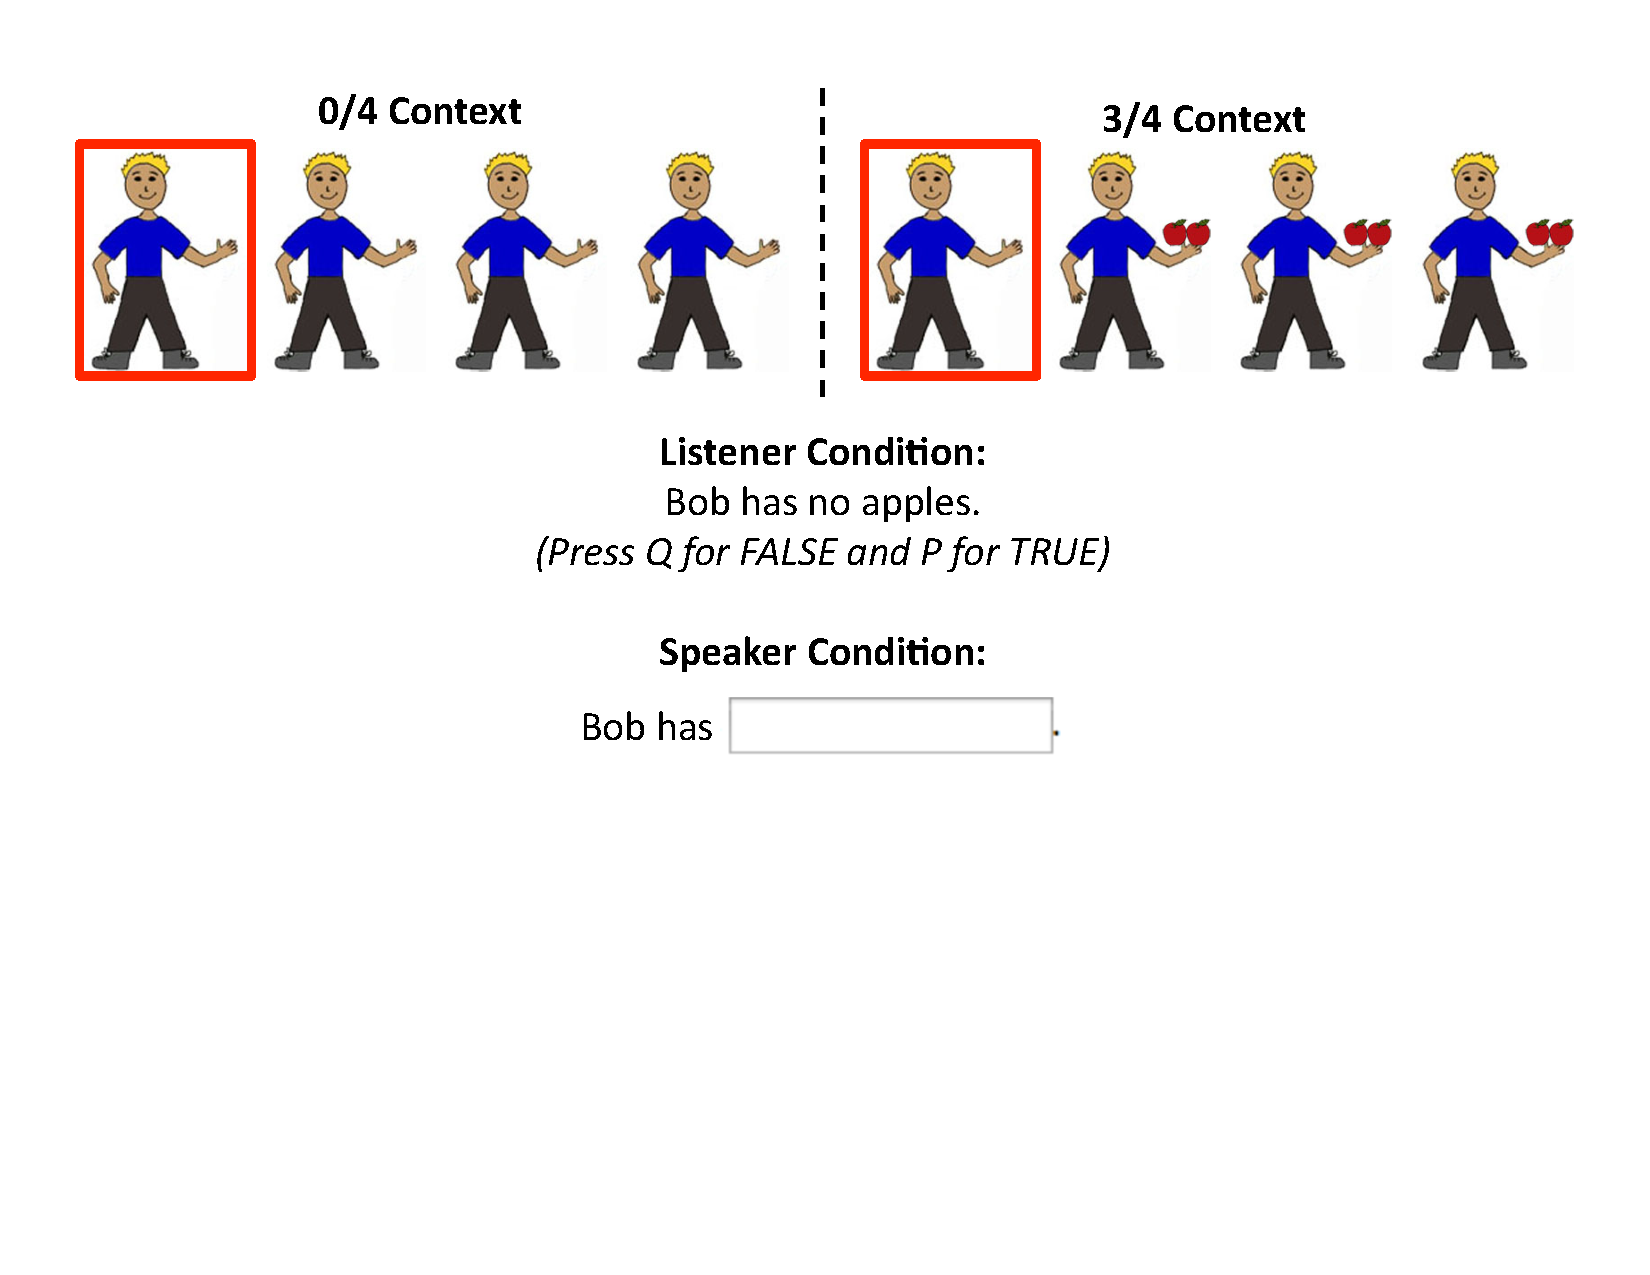
\includegraphics[width=6in]{figures/trialfig.pdf}
\caption{\label{fig:trial} An example of a true negative trial with a 0/4 context (left) and a 3/4 context (right).  The sentence ``Bob has no apples'' in the 0/4 context is both uninformative (because the sentence is true of all of the characters) and irrelevant (because apples are not present in the context), whereas the same sentence in the 3/4 context is informative and relevant. }
\vspace{-5mm}
\end{center} 
\end{figure}

Thirty-two trial items were created in which characters were shown holding either two of the same common, recognizable objects (``target items''; e.g., two apples), or holding nothing.  Within each trial, all characters were identical except for the presence or absence of objects; characters varied in appearance (e.g. skin tone, hair color, clothing, gender) across trials. Our previous work indicates that the results reported here are robust to a number of changes to the stimuli, including whether the context characters varied in appearance or not \cite{nordmeyer2014}. 

Each participant saw trials in which different proportions of characters were holding target items (context condition).  These contexts showed $\frac{0}{4}$, $\frac{1}{4}$, $\frac{2}{4}$, $\frac{3}{4}$, or $\frac{4}{4}$ of the characters holding objects. The order of characters was shuffled on each trial, with the referent of the sentence appearing in a random position. 

Participants in the speaker condition saw each image paired with an incomplete sentence (e.g. ``[NAME] has $\rule{3cm}{0.15mm}$.''). In half of the trials, the highlighted character was holding target items (``item trials''), and in half of the trials, the highlighted character was holding nothing (``nothing trials'').  The experiment was fully crossed such that target characters appeared with or without target items an equal number of times in each context type.  

Participants in the listener condition saw the same set of images.  On each trial a sentence of the form ``[NAME] [has/has no] [ITEM]'' appeared.  Half of the sentences were positive and half were negative (sentence type), and they were paired with pictures such that half were true and half were false (truth value), resulting in four possible trial types (true positive, true negative, false positive, and false negative).  Because true positive and false negative sentences cannot occur in a $\frac{0}{4}$ context (i.e. the referent must have the target item in these trials), and true negative and false positive sentences cannot occur in a $\frac{4}{4}$ context, each trial type occurred in four possible contexts.  The experiment was fully crossed, with participants receiving eight true positive, eight false positive, eight true negative and eight false negative sentences distributed equally across context types in a randomized order over the course of the study.  

\subsection{Procedure}

Participants were first presented with a brief overview screen which explained that they would play a language game.  Once participants accepted the task, they were randomly assigned to either the speaker condition or the listener condition, and saw a more detailed instructions screen which explained the task and informed them that they could stop at any time. The speaker and listener conditions of the experiment can be viewed at \url{https://langcog.stanford.edu/expts/AEN/negatron_production2/negatron.html} and \url{https://langcog.stanford.edu/expts/AEN/negatronv20/negatron.html}, respectively.

In the speaker condition, participants saw an array of four pictures on each test trial: The target pictures and three context pictures presented in a random horizontal arrangement.  Participants were told to look at these pictures for four seconds, at which point a red box appeared around one of the pictures.  One second later, an incomplete sentence appeared.  Participants were told to finish the sentence (by typing into a small text box) using only a few words, in a way that would help someone else identify the character in the red box if they saw the pictures in a different order.

In the listener condition, participants first saw eight positive sentence practice trials with feedback about incorrect responses before beginning the test trials. In each test trial, participants saw an array of four pictures presented in a random horizontal arrangement.  Participants were told to look at these pictures for four seconds, at which point a red box appeared around one of the pictures.  One second later, a sentence about that picture appeared.  Participants were told to read the sentence and respond as quickly and accurately as possible with a judgment of whether it was true or false when applied to the highlighted picture.  We recorded reaction times for each trial, measured as the time from when the sentence was presented to the moment when the response was made.
  
\subsection{Data Processing} 
  
We excluded 18 participants who did not list English as their native language and two participants from the listener condition for having an overall accuracy below 80\%, leaving a total of 469 participants for analysis (186 in listener condition, 283 in speaker condition). 

In the speaker condition, we coded participant's productions. Affirmative responses labeling the target feature were coded as ``positive'' (e.g., ``apples,'' ``two apples,'' ``red apples,'' etc.).  Responses negating the target feature (e.g., ``no apples'') were coded as ``negative.''  All other responses (e.g. descriptions of the characters' clothing or hair color) were coded as ``other.''  Codes were hand-checked to ensure that label synonyms or spelling errors were coded correctly.

In the listener condition, we excluded trials with RTs greater than 3 standard deviations from the log-transformed mean, a criterion established in our previous experiments \cite{nordmeyer2014}.  

To predict responding in the listener condition, we used productions from the speaker condition. We calculated the proportion of positive sentences describing characters who possessed target items, and the proportion of negative sentences describing characters with nothing, creating probability distributions for true positive and true negative utterances in each context.  We then used this distribution to calculate the surprisal of hearing a true positive or true negative sentence for each context. Surprisal is an information-theoretic measure of the amount of information carried by an event (in this case, the amount of information conveyed by a sentence); in prior work on sentence comprehension it has been used successfully as a linking hypothesis between production probabilities and reaction times \cite{levy2008}. Surprisal (or ``self-information'' $I$) for a sentence $s$ is defined as

\begin{equation}
\label{eq:surprise}
I(s) = -\log(P(s)).
\end{equation}

\section{Results}

\subsection{Speaker Condition}

\begin{figure}[t]
\begin{center} 
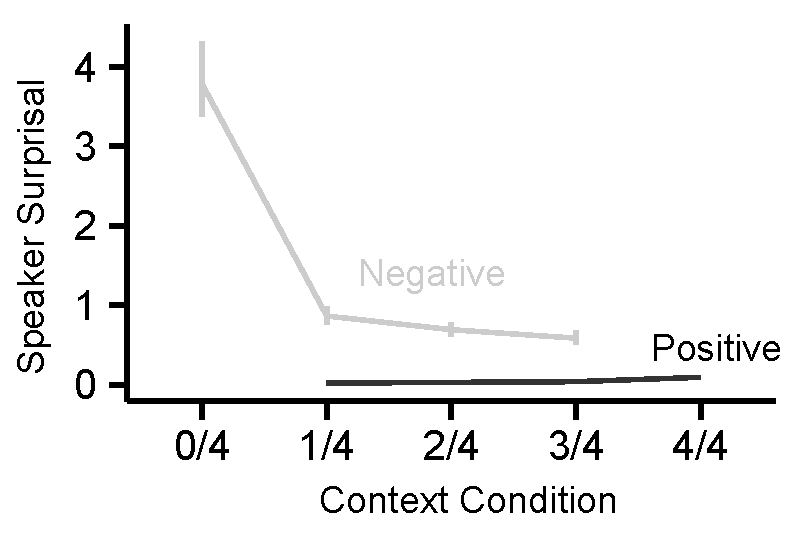
\includegraphics[width=3in]{figures/surprisals_mod.pdf}
\caption{\label{fig:speakersurprise} Surprisal for true positive and true negative sentences across different contexts. Negative sentences are shown in grey, and positive sentences in black.  The context is notated by a fraction representing the number of characters in the context who held target items. Error bars show 95\% confidence intervals computed by non-parametric bootstrapping.  }
\end{center} 
\end{figure}

Participants were much more likely to produce negation when the target character was not holding anything (nothing trials), and produced negative sentences very rarely when the target character was holding target items (item trials).   Consistent with our hypothesis that speakers will produce negative sentences that are relevant (i.e. negating a salient feature of the context), negative sentences were produced very rarely on nothing trials in the $\frac{0}{4}$ context (e.g. ``no apples'' was a rare production on trials where there weren't any apples in the context; see Figure \ref{fig:trial}), but became much more common on nothing trials in the $\frac{1}{4}$ context.  In line with our hypothesis that speakers will produce informative utterances (i.e. produce sentences that are maximally effective at identifying the referent), participants in the speaker condition were increasingly likely to produce negation as the number of characters with target items increased, with the  $\frac{3}{4}$ context eliciting the highest production of negation.  

To evaluate the reliability of these patterns, we fit a binomial mixed-effects model to test the effect of trial type and context on the probability of producing a negative sentence.  To test the quantitative effects of context, we coded this variable as numeric, e.g. the proportion of characters in the context with target items.  In addition, because the difference between the  $\frac{0}{4}$ and the  $\frac{1}{4}$ contexts was so striking, we created a dummy code to separately test for the effects of the  $\frac{0}{4}$ context compared to all of the other contexts.  All mixed-effects models used the maximal convergent random effects structure and were fit using the lme4 package version 1.1-7 in R version 3.1.2.  The model specification was as follows: \texttt{negation $\sim$ context~$\times$~trial type + dummy context + (1~\textbar~subject) +  (1~\textbar~item)}.  Raw data and analysis code can be found at \url{https://github.com/anordmey/negatron}.

\begin{table}[t]
\caption{\label{tab:speakermodel} Coefficient estimates from a binomial mixed-effects model predicting speaker's productions in different contexts.}
\begin{center}
% \small\addtolength{\tabcolsep}{-5pt}
\begin{tabular}{rrrrr}
  \hline
 & Coefficient & Std. err. & $z$ & $p(|z|)$ \\ 
  \hline
Intercept & -8.30 & .82 & -10.12 & $<$.001 \\ 
  Context & .01 & 1.15 & .01 &  0.99 \\ 
  Trial Type (nothing) & 7.12 & .81 & 8.76 & $<$.001 \\
  Dummy context ($\frac{0}{4}$) & -4.74& .29 & -16.30 & $<$.001 \\ 
  Context $\times$ Trial Type & 2.18 & 1.17 & 1.86 & 0.063 \\
   \hline
\end{tabular}
\vspace{-1.5cm}
\end{center}
\end{table}

All model coefficients are shown in Table \ref{tab:speakermodel}.  Main effects of trial type and dummy context confirm that participants were much more likely to produce negative sentences on nothing trials (i.e. trials where the target character held nothing) and much less likely to produce negation in the $\frac{0}{4}$ context.  A marginally significant interaction between context and trial type suggests that there is a linear effect of context on nothing trials even after accounting for the effect of the $\frac{0}{4}$ context.  Following up on this finding in an exploratory analysis, we fit a model to only the data on nothing trials in the $\frac{1}{4}$, $\frac{2}{4}$, and $\frac{3}{4}$ contexts, and found a significant linear effect of context on the production of negation ($\beta= 2.28$, $p< .001$), suggesting that negative sentences were more likely to produced in contexts where they were more informative.  

Figure \ref{fig:speakersurprise} shows the surprisal of true positive (i.e. descriptions of the target noun on item trials) and true negative (i.e. negations of the target noun on nothing trials) sentences.  Consistent with our predictions, surprisal is highest for true negative sentences in the $\frac{0}{4}$ context, and surprisal for true negative sentences decreases as the number of context characters with target items increases.

\subsection{Listener Condition}

\begin{figure}[t]
\begin{center} 
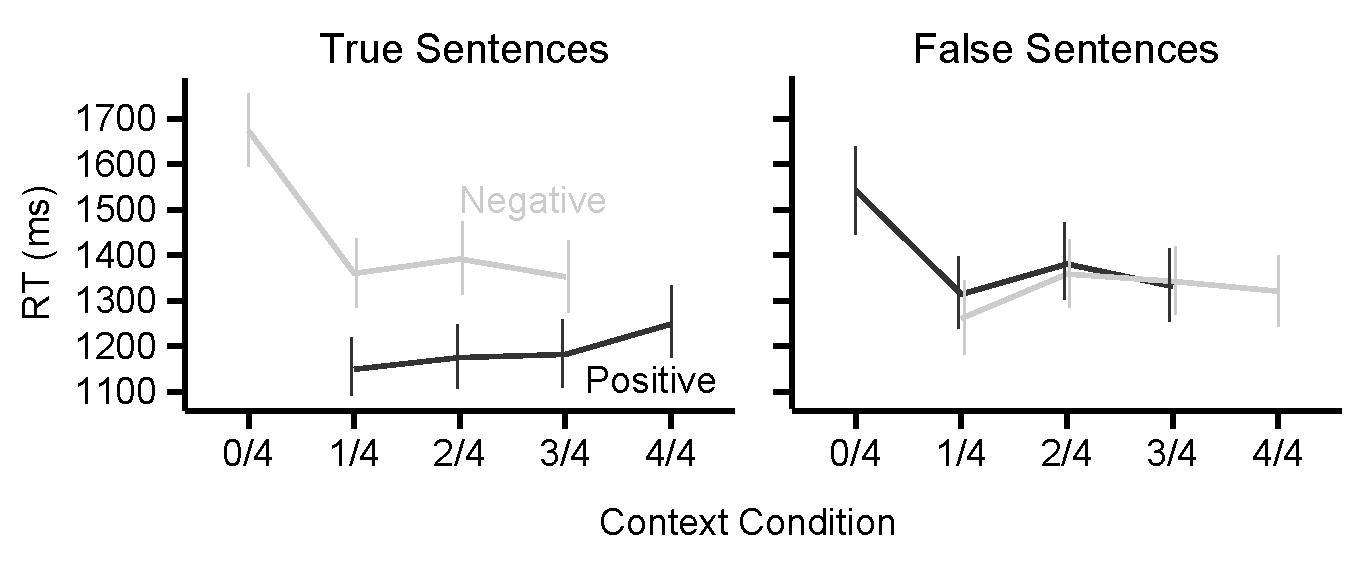
\includegraphics[width=5in]{figures/rts_mod.pdf}
\caption{\label{fig:listenerrt} Reaction times for each trial type across different conditions. Responses to true sentences are shown on the left, and false sentences are shown on the right.  Negative sentences are shown in grey, and positive sentences in black.  The context is notated by a fraction representing the number of characters in the context who held target items. Error bars show 95\% confidence intervals computed by non-parametric bootstrap.}
\end{center} 
\end{figure}

Participants were fastest to respond to true positive sentences, and slowest to respond to true negative sentences, replicating previous findings \cite{hclark1972}.  Listeners' responses to true negative sentences mirrored the surprisal of true negative sentences in the speaker condition, with participants responding slowest to true negatives in the $\frac{0}{4}$ context.  The same pattern was seen in response to false positive sentences, suggesting that listeners expect speakers to describe relevant features of the context even when the sentence is false (see Figure \ref{fig:listenerrt}).  

We fit a linear mixed-effects model to examine the interaction between sentence type (positive or negative), truth value (true or false), and context as predictors of reaction time. The model specification was as follows: \texttt{RT $\sim$ sentence~$\times$~truth~$\times$~context + (sentence~\textbar~subject) +  (sentence~\textbar~item)}.  Significance was calculated using the standard normal approximation to the $t$ distribution \cite{barr2013}.

All model coefficients are shown in Table \ref{tab:listenermodel}. In addition to main effects of sentence type and truth value, the model showed an interaction such that true positive sentences elicited the fastest responses and true negative sentences elicited the slowest responses. The model showed a significant negative linear effect of context, with reaction times decreasing as the proportion of characters with target items increased. A significant three-way interaction between sentence type, truth value, and context indicates that this pattern was driven primarily by responses to true negative sentences, however, with true positive and false negative sentences showing a smaller positive linear effect of context.  

\begin{table}[t]
\caption{\label{tab:listenermodel} Coefficient estimates from a mixed-effects model predicting listeners' reaction times in response to sentences in different contexts.}
\begin{center}
% \small\addtolength{\tabcolsep}{-5pt}
\begin{tabular}{rrrr}
  \hline
 & Coefficient & Std. err. & $t$ \\ 
  \hline
Intercept & 1482 & 39 & 37.57 \\ 
  Sentence (Negative) & -204 & 36 & -5.61  \\ 
  Truth (True) & -369 & 36 & -10.29 \\
  Context & -238 & 44 & -5.44 \\ 
  Sentence $\times$ Truth & 686 & 51 & 13.42 \\
  Sentence $\times$ Context & 311 & 62 & 5.05 \\
  Truth $\times$ Context & 366 & 61 & 5.97 \\
  Sentence $\times$ Truth $\times$ Context & -835 & 88 & -9.52 \\
   \hline
\end{tabular}
\vspace{-1.5cm}
\end{center}
\end{table}


\subsection{Predicting Listeners with Speakers}

\begin{figure}[t]
\begin{center} 
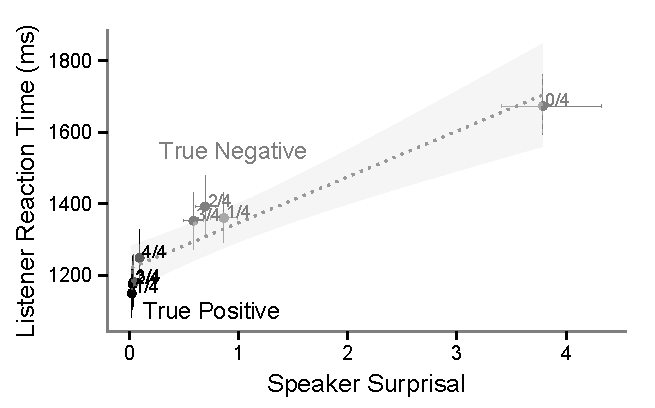
\includegraphics[width=4in]{figures/production_rts_mod.pdf}
\caption{\label{fig:scatter} Reaction times in the listener condition plotted by surprisal in the speaker condition; each point represents a measurement for sentence type and context. Error bars on the horizontal and vertical axes represent 95\% confidence intervals on their respective measures.}
\end{center} 
\end{figure}

To test the hypothesis that processing times are a function of listeners' expectations about what a speaker will say, we regressed the mean reaction time in response to true positive and negative utterances in each condition against the surprisal for the same utterances (Figure \ref{fig:scatter}).  There was a significant positive relationship between surprisal and reaction time for true negative sentences, $r^2=.90$, $p<.001$, supporting our prediction that the effects of context on reaction time reflect differences in how speakers would describe the same stimuli.  

\section{General Discussion}

What makes negation hard to process? While previous work has proposed that processing negative elements is especially difficult because of features intrinsic to negation, our work here suggests instead that general pragmatic mechanisms are likely responsible. Negative sentences presented without context are uninformative and irrelevant; thus, they are unlikely to be produced by speakers. In turn, listeners respond to these unlikely utterances with increased processing times. In contexts where negation is more informative and relevant, processing costs are lower. Overall, this evidence supports a Gricean interpretation of the processing of negation.

While previous work has shown that contextual factors facilitate the processing of negation \cite{wason1965,nieuwland2008,dale2011}, our findings here go further. First, and most importantly, by using actual language productions as the predictor of processing difficulty, our work strongly implicates specifically pragmatic (rather than representational) factors. Second, rather than treating pragmatics as a black box, we show that two different components---informativeness and relevance---each contribute to the relative (un-)likelihood of hearing a negation. 
% Informativeness predicts that speakers should produce utterances that are maximally helpful in allowing the listener to identify the referent of a sentence.
% ; our data suggests that speakers are increasingly likely to describe a character by negating the target feature as the number of context characters \emph{with} the target feature increases.  
% Furthermore, the low probability (and corresponding slow reaction time) of participants producing true negative sentences in the $\frac{0}{4}$ context suggests that speakers are unlikely to produce negation unless there is a relevant feature to negate.

Our work here also uses surprisal, an information-theoretic measure of processing difficulty, as the linking hypothesis between speaker probabilities and reaction times \cite{levy2008}. Although this link has substantial support in the realm of syntactic processing \cite{demberg2008,boston2008}, to our knowledge, our findings are the first example of using surprisal over sentence-level pragmatic expectations, rather than word-level syntactic expectations. This success suggests that, in concert with the appropriate predictive models, surprisal theory could be productively applied to the prediction of processing difficulty beyond the level of syntax. 

Although our focus here was on negation, our findings have implications for sentence processing more generally.  Debates about the effects of pragmatics on linguistic processing exist in other domains, such as the processing of scalar implicatures \cite<the pragmatic inference that e.g., ``some'' implicates ``some but not all'';>{huang2009, huang2011, grodner2010}.  \citeA{tomlinson2013} provide an informative comparison between scalar implicature and negation, presenting mouse-tracking trajectories for each. Their negation data show the same pattern of processing difficulties we observe, and critically, their data on the processing of underinformative ``some'' utterances look almost identical. We hypothesize that, in both cases, participants' processing difficulty is a function of the violation of their pragmatic expectations.

In sum, our findings here suggest that a large part of the processing difficulties of negative sentences arise from the relative pragmatic felicity of negation in context. They do not rule out the possibility that there is some cost to processing an additional logical element, but this processing cost would have to be quite small with respect to the magnitude of the effects we observed (and previous measurements). This finding leads us to the following conclusion: When logical words are used in a communicative context, we have no difficulty understanding them.

\subsection{Author Contributions}
Both authors developed the study concept and contributed to the study design.  Data collection was conducted by A. E. Nordmeyer.  A. E. Nordmeyer performed the data analysis and interpretation under the supervision of M.C. Frank.  Both authors contributed to the development of the manuscript and approved the final version of the manuscript for submission.

\subsection{Acknowledgments}
This work supported by the NSF GRFP and ONR N00014-13-1-0287.

%  show the same mouse-tracking patterns in response to underinformative scalar implicatures as well as underinformative negative utterances.  

% We believe that formal models of pragmatics can provide insight into these debates and, more generally, into the role that pragmatic context plays in linguistic processing. 

% One contribution of our work here is that we use language production behavior to provide a strong operational definition of pragmatics.  Building on recent 

 % modeling work quantifies pragmatic reasoning based on the assumption that speakers are informative---they will produce utterances that pick out smaller subsets of the context, leaving as little ambiguity as possible for the listener \cite{frank2012,goodman2013}.  By this definition, negative sentences become more informative as the number of characters in the context increases.  This prediction is reflected in our results: Speakers were more likely to use negation in contexts where more people possessed the negated item.  

% We also found that both speakers' and listeners' behavior was strongly influenced by the presence of any target items in the context.  Speakers were much less likely to produce a negative utterance when none of the characters in the context possessed target objects; similarly, listeners took much longer to respond to these sentences than any of the other contexts.  We saw the same pattern in listeners' responses to false negative sentences.  These findings are consistent with relevance theory \cite{sperber1986}, as well as the idea that a speakers' utterances are influenced by the ``Question Under Discussion'' \cite{roberts1996}.  In addition to being uninformative, a sentence such as ``Bob has/has no apples'' in a context where none of the characters have apples is very strange, because ``apples'' is not a relevant feature of the context.  We interpret this finding as evidence for the role of relevance in producing and processing speech; in addition to being uninformative, these sentences might have incurred additional processing costs due to the mention of an unexpected topic.    

%Our analyses focused on true sentences, because of our interest in exploring participants' expectations about how an informative speaker should behave.  Due to the nature of our task, participants in the listener condition likely expected some of the sentences to be false, but it is not clear what constitutes an ``informative'' false sentence.  Our listener data replicate an interaction between sentence type and truth value that is seen frequently in literature on sentence verification tasks \cite{hclark1972}, with false positive sentences showing a similar pattern as true negative sentences.  




% These were contexts in which negation was informative (i.e., identified a narrower subset of the context) and relevant (i.e., the negated item was present in the context).  This pattern was also consistent with our Gricean hypothesis that the processing cost of negation is due to general pragmatic principles about how listeners expect speakers to behave.  

% In conversation, in contrast, negative sentences are often produced when some strong expectation has been violated, making the negation both informative and relevant. Congruent with that impression, 

% Our participants were faster to respond to negative sentences in contexts where speakers were more likely to use negation to describe the same stimuli. 

%We suggested a Gricean account of these data: The processing cost of negation is related to the degree to which it violates expectations about communication in context. In our studies, by changing the proportion of people in the context who held a target item, we systematically manipulated participants' contextual expectations.  We found a parametric relationship between the strength of the context and reaction times, and this relationship was well fit by participants' descriptions of the stimuli in different contexts.


 
 % and slower processing times.  


\bibliographystyle{apacite}

\setlength{\bibleftmargin}{.125in}
\setlength{\bibindent}{-\bibleftmargin}

\bibliography{negation}

\end{document}


%Maybe move some of this to the GD
%What is the mechanism by which context influences the processing of negation?  We propose that negative sentences are more informative in contexts that set up a strong expectation that is violated. If the processing cost of negation is pragmatic, then more informative negative sentences should elicit smaller reaction times. How should we quantify informativeness in context? Recent modeling work quantifies pragmatic reasoning in simple experimental contexts \cite{frank2012,goodman2013}. The assumption underlying this work is that speakers are informative---they will produce utterances that will pick out smaller subsets of the context, leaving as little ambiguity as possible for the listener.  We use this definition of informativeness to provide a quantitative interpretation of our hypothesis.

%MOVE THIS:
%To link pragmatic expectations to reaction time, we assume that reaction time is proportional to \emph{surprisal}. Surprisal is an information-theoretic measure of the amount of information carried by an event (in this case, an utterance in some context) based on its probability. Surprisal has been used effectively to predict reaction times from probabilistic models \cite{levy2008}; in this work, we directly measure the probability of an utterance occurring by eliciting descriptions of our stimuli from our participants.